\documentclass{beamer}
\usepackage{tikz}

\begin{document}
    \begin{frame}
        \centering
        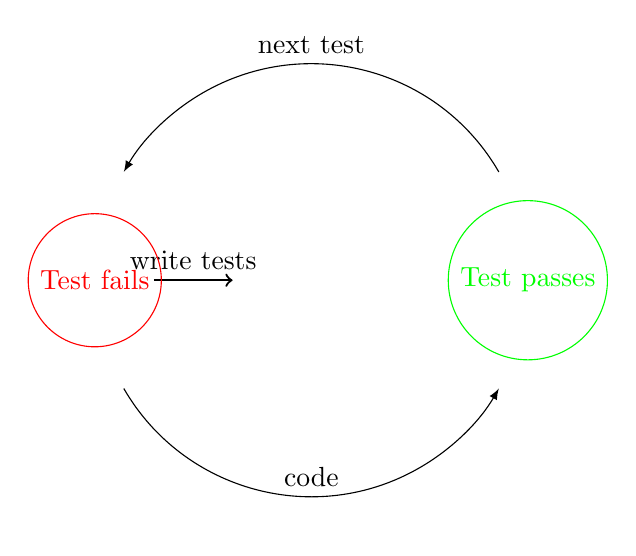
\begin{tikzpicture}
            \def \n {2}
            \def \radius {2.75cm}
            \def \margin {30}
            \draw[->,thick] (-2,0) -- (-1,0) node[midway, above] {write tests};
            \foreach \s/\A/\C/\N in {1/Test passes/green/next test,2/Test fails/red/code}
            {
              \node[draw, circle,\C] at ({360/\n * (\s - 1)}:\radius) {\A};
              \draw[->, >=latex] ({360/\n * (\s - 1)+\margin}:\radius) arc ({360/\n * (\s - 1)+\margin}:{360/\n * (\s)-\margin}:\radius) node[midway, above] {\N};
            }
        \end{tikzpicture}
    \end{frame}
\end{document}